\documentclass[a4paper]{article}

\usepackage{amsmath}

%\usepackage[citestyle=authoryear]{biblatex}
%\addbibresource{references.bib}

\title{Identification of the open loop dynamics of a bicycle-rider system
under manual control}
\author{Jason K. Moore and Mont Hubbard}
\date{\today}

\begin{document}

\maketitle

\section{Introduction}

Today's dynamical experiments are capable of delivering a staggering amount of both kinematic and
kinetic data from complex dynamical systems. Such large amount of data lends
itself to data driven modeling approaches that can potentially provide more
predictive models than the traditional buidling blocks of dynamical models using first principles.
These data driven models can also give insight into the defecencies of first
principles models. Here we explore the bicycle-rider system and discuss both
traditional models and data driven models.

Bicycles and the bicycle-rider system have been modeled by a variety of models,
both simple \cite{Timoshenko1948} and complex \cite{Sharp1971}. Many of
today's studies rely on the benchmarked Whipple model, with or without the
addition of tire models, for analytical studies of the system and simulation
comparisons. The Whipple bicycle model is regarded as a highly predictive model
of the bicycle-rider system and is constructed from first principles, yet very
little experimental data proves that the Whipple model is in fact a robust
model for the open loop dynamics of the bicycle-rider system. There are also a
variety of popular motorcycle models (Sharp, Cosalter) that may be a good
predictor of the system dynamics, but no one has attempted to verify that for a
bicycle-rider system. The author is only aware of two significant experimental
attempts at validating the model. The most cited, Kooijman, shows that the
Whipple model is predictive of a riderless bicycle in a gymnasium and on
a treadmill for speeds in its predicted stable speed range, 4-6 m/s. Cain shows
that the Whipple model reduced to a linear steady turn can predict the
kinematics, but is not so good at predicting the rider's input torque.

It is worth noting that Eaton, James, \ldots, worked to identify models of
motorcycles with varying degrees of results. Talk more about these. %DELETE????

Two remedy this,%remedy what? shoudl say like "remedy this issue of the Whipple model not being proven in real life
we have collected a large set of mostly time history data from
an instrumented bicycle which includes some of the most important kinematic and
kinetic variables describing the bicycle-rider motion from three different
riders on the same bicycle for a variety of maneuvers and speeds. %sentence way too long, also doesn't really make sense.
These experiments generated about 1.7 million time samples from each of about 30
sensors collected at 200 hertz (representing about 2.4 hours of real time).

\section{Experimental Design}

\subsection{Instrumented Bicycle}
We developed an instrumented bicycle that had a unique combination of sensors
for dynamic measurements that are known to be important indicators for the
bicycle-rider system motion. The bicycle's primary design criteria were as
follows:

\begin{itemize}
  \item It should be sized for our intended riders: average adult males in
    Davis California. %delete probably, not really relevant or good to include
  \item The rider's biomechanical movement, including pedaling, should be
    restricted as much as possible so that the Whipple model's rigid rider
    assumption is more probable.
  \item It %the bicycle or bike instrumentation
  should accurately measure the fundamental kinematics of the bicycle:
    three dimensional rates and orientations of the bicycle rear frame, front
    frame, and wheels.
  \item It should accurately measure the rider's applied steering torque.
  \item It should accurately measure an applied lateral disturbance force to
    the bicycle frame.
  \item Experiments could be performed on open road or on a treadmill.
\end{itemize}

With these criteria in mind we constructed a bicycle with an electric
propulsion system and rigid rider harness and an assortment of sensors. The
rear frame 3D angular rates and a 3D point acceleration were measured with a
VectorNav VN-100 interial measurement unit, the rear frame roll angle was
measured with a rotary potentiometer mounted to a small lightweight trailer,
the steer angle was measured with a rotary potentiometer, the axial torque in
the steer tube by a Futek 150 in-lb (±17 Nm) TFF350 torque sensro, the lateral
perturbation force by a load cell 100 lb force load cell (Interface SSM-100),
the angular rate about the steer axis of the front frame by a rate gyro Single
axis rate gyro (Silicon Sensing CRS03-04S), and the rear wheel angular rate by
a dc generator.

%\begin{figure}
  %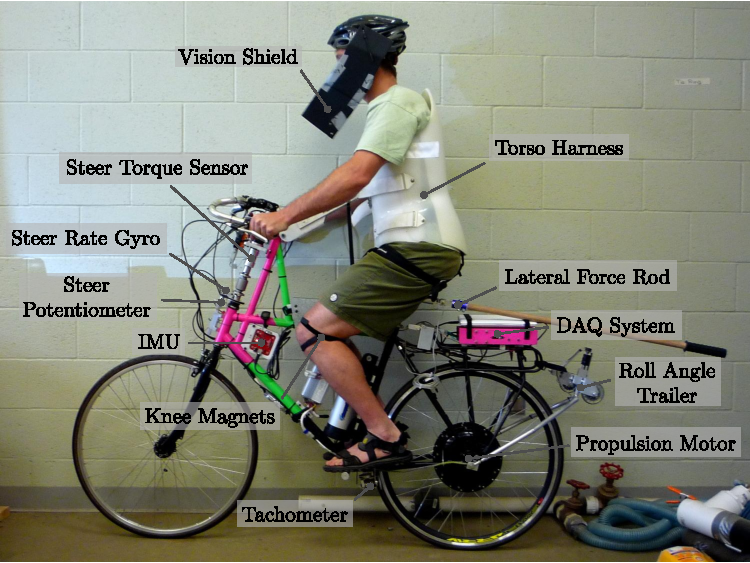
\includegraphics[width=5in]{figures/instrumented-bicycle.pdf}
  %\caption{The instrumented bicycle with on of the rider's seated in the
  %harness.}
%\end{figure}

\subsection{Experiments}
We recorded data from a variety of experiments \cite{Moore2012} but %delete

the analysis herein focuses on the two maneuvers which we call \emph{Heading
Tracking} and \emph{Lateral Deviation Tracking}. Our definitions of these are:

\begin{description}
  \item[Heading Tracking]
    The rider was instructed to simply balance the bicycle and keep a
    relatively constant heading while focusing their vision at a point in the
    far distance.
  \item[Lateral Deviation Tracking]
    The rider was instructed to focus on a straight line that was marked on the
    ground and to attempt to keep the front wheel on the line.
\end{description}
%you could technically just make these part of the above paragraph and that would save you line space.

Both tasks were performed with and without the application of a manually
applied lateral perturbation forces just below the seat. The forces were
applied randomly in direction and time during the trials. Each maneuver was
performed on both a 1 meter wide treadmill and an open gymnasium floor. See
\cite{Moore2012} for more details.

\section{Data}

The physical parameters (geometry, mass, center of mass, and moments of
inertia) of both the bicycle and the rider were estimated using the methods in
\cite{Moore2012} and \cite{Yeadon1990}, respectively %respective to what? bicycle and rider? or the different physical parameters?
. The bicycle was measured
to get accurate estimates of the parameters used in the benchmark bicycle. %weird sentence. reduce "bicycle" to one time if you can
The
combined inertial properties of the bicycle rear frame and the rider were
computed with standard methods. Two open source software packages, yeadon
\cite{Dembia2011} and BicycleParameters \cite{Moore2011} manage and process the
data physical parameter data. %watch tense

% TODO: Add a table of the whipple model parameters for the three riders

Before each day of testing, data was collected for the system's sensors for
calibration purposes. Then for each trial a set of meta data and raw time
series were collected from the bicycle's onboard DAQ system. This data was
stored in a HDF5 database for easy querying and retrieval in the data analysis
step. The raw data was then processed to obtain the desired time histories
defined by the Whipple model coordinates:

\begin{table}
  \begin{tabular}{lll}
    Variable                                            & Description                                    & Units \\
    \hline
    $v$                                                 & wheel center speed magnitude                   & m/s \\
    $\delta,\phi,\psi$                                  & steer, roll and yaw angles                     & rad \\
    $\dot{\delta},\dot{\phi},\dot{\psi},\dot{\theta}_B$ & steer, roll, yaw, and rear wheel angular rates & rad/s \\
    $T_\delta,F_{c_l}$                                  & steer torque, lateral perturbation force       & NM, N
  \end{tabular}
\end{table}

Before identification computations we subtracted the means over time of the
signals that were generally symmetric about zero. For some of the pavilion
runs, this may have actually introduced a small bias, as the short duration
runs with unbalanced perturbations may not have zero mean. This was repeated 
for all the signals except the lateral force.

For the following analysis%what analysis?
, all of the signals were filtered with a second order
low pass Butterworth filter at 15 Hz. 

% TODO: example plot of the signals

The experimental data was collected on seven different days and amounted to
about 600 individual trials with three different riders. We used X of the 
runs for the following analysis.

\section{System Identification}

- data processing
- state space form
- canonical form

The overarching goal in the research project which this work was a part of was
to identify the manual control system employed the rider, but the schemes we
used for that identification relied on an accurate plant model
\cite{Moore2012}. We ended up approaching this in a similar fashion to
\cite{Eaton1973} and attempted to identify the plant, i.e. the open loop
bicycle and rider dynamics, first followed by an identification of the control
system. The question arises as to what the plant and controller consist of. In
this case, we consider the plant to include the passive or open loop model of
the bicycle combined with the rider's biomechanics and the controller to be
some makeup of the human brain which takes sensory inputs, has time delays, and
sends outputs for muscular control.

This two part process was not originally thought to be needed and we started
with the identification of the control system assuming the Whipple model would
be adequate for the open loop dynamics. But my preliminary attempts at
identifying the controller with the Whipple model in place showed that the
plant always under-predicted the steer torque needed for a given measured
trajectory. This lead me into the exploration of the validity of the Whipple
model.

There is actually very little experimental validation of the open loop dynamics
of the bicycle, with \cite{Kooijman2006} being one of the better studies. But
his study was limited to a riderless bicycle in a narrow speed range where the
bicycle was stable. Taking the validity of first principles models like this
for granted can potentially lead to inaccurate conclusions. In our case, it
resulted in erroneous early estimations of the controller parameters. As
pointed out by many, in particular the motorcycle researchers, there is very
good reason to question some of assumptions in the various first principles
models. The main questionable assumption being knife-edge no side-slip wheels,
especially when under a rider's weight.  And secondly, the rider's biomechanics
have much more influence and coupling to the bicycle than the motorcycle, which
must be accounted for.

Before I proceed, it is important to emphasize the difference in identifying a
model that best predicts the data and identifying physical parameters in a
model structure that cause the predictions to best fit the measured data. In
the first case, it is somewhat easy to fit a model to input and output data. By
increasing the order of the model and thus the number of free parameters one
can theoretically fit every data point. This is most evident in the
over-fitting of a linear trend with that of a higher order polynomial. It still
often takes human intuition and reasoning to limit the order of the system to
something that represents the true relationships between the variables. But
even in this case, the individual meaning of the resulting identified
parameters of a black box system may have little apparent connection to the
known first principles laws we are familiar with and trust. In dynamics, we
often want to know how well our first principles models predict the measured
motion and secondly we'd like the ability to identify parameters, particularly
ones we are uncertain of in the first principles models, from the measured
data. Accurately identifying model parameters is much more difficult task,
because noises, both process and measurement, have to be accounted for to get
repeatable and accurate estimates of the parameters. I have had good success
with finding models that predict the data but little success with explicit and
accurate parameter identification in the following analyses. There is great
room for improvement in the parameter identification if the noise issues are
better managed. %this paragraph can be truncated. Either put some of this in the intro, or delte a lot of it.

\section{Structured Black Box State Space Identification}

The open loop dynamics of the bicycle-rider system can be described using many
models \cite{Astrom2005}, \cite{Limebeer2006}, and \cite{Meijaard2007} ). The 
benchmarked Whipple bicycle model \cite{Meijaard2007}
provides a minimalistic standard base model in a manageable analytic framework capable
of describing the essential dynamics such as speed dependent
stability, steer and roll coupling, and non-minimum phase behavior. 

The non-linear Whipple model is a 4th order system with roll angle, steer
angle, roll rate, and steer rate selected as the independent states and with
roll and steer torques as the generalized forces and system inputs. In place 
of the roll torque input, the model is extended to include a lateral
force acting at a point on the frame to provide a new input, accurately
modelling imposed lateral perturbations (see \cite{Moore2012} for details). 
We also examine a second candidate model which adds the
inertial effects of the rider's arms to the Whipple model, also described in
\cite{Moore2012}. This model was designed to more accurately account for the
fact that the riders were free to move their arms with the front frame of the
bicycle. This model is similar in fashion to the upright rider in
\cite{Schwab2010a}, but with slightly different joint definitions. Constraints
are chosen so that no additional degrees of freedom are added, keeping the
system both tractable and comparable to the benchmarked Whipple model.

We then make the basic assumptions that the model is (1) linear, (2) is fourth
order, and (3) we can measure the states and inputs directly while the system
is under closed loop control by the rider. We then employ the direct
identification approach to identify the plant.

During all of the experiments there are at least two measured external
(exogenous) inputs: the steer torque and the lateral force. Both inputs are
generated manually, the first from the rider and the second from the person
applying the pulsive perturbation. The outputs can be any subset of the
measured kinematical variables or combinations thereof, we selected the roll
and steer angles and rates. The problem can then be formulated as follows:
given the inputs and outputs of the system and some system structure, what
model parameters give the best prediction of the output given the measured
input? This a classic system identification problem.

The ideal linear Whipple model can be generally be described with the following
continuous state space description:

\begin{align}
  \dot{x}(t) & =
  \mathbf{F}x(t) + \mathbf{G}u(t)\\
  \begin{bmatrix}
    \dot{\phi} \\
    \dot{\delta} \\
    \ddot{\phi} \\
    \ddot{\delta}
  \end{bmatrix}
  & =
  \begin{bmatrix}
    0 & 0 & 1 & 0\\
    0 & 0 & 0 & 1\\
    a_{\ddot{\phi}\phi} & a_{\ddot{\phi}\delta} &
    a_{\ddot{\phi}\dot{\phi}} & a_{\ddot{\phi}\dot{\delta}}\\
    a_{\ddot{\delta}\phi} & a_{\ddot{\delta}\delta} &
    a_{\ddot{\delta}\dot{\phi}} & a_{\ddot{\delta}\dot{\delta}}
  \end{bmatrix}
  \begin{bmatrix}
    \phi \\
    \delta \\
    \dot{\phi} \\
    \dot{\delta}
  \end{bmatrix}
  +
  \begin{bmatrix}
    0 & 0 \\
    0 & 0\\
    b_{\ddot{\phi}T_\delta} & b_{\ddot{\phi}F_{c_l}}\\
    b_{\ddot{\delta}T_\delta} & b_{\ddot{\delta}F_{c_l}}
  \end{bmatrix}
  \begin{bmatrix}
    T_\delta\\
    F
  \end{bmatrix}\\
  \eta(t) & = \mathbf{H}x(t)\\
\end{align}

where $\eta(t)$ are the outputs and $\mathbf{H}$ is the identity matrix.

Assuming that this model structure can adequately capture the dynamics
of interest of the bicycle-rider system, our goal is to accurately
identify the unknown parameters $\theta$ which are made up of the
unspecified entries in the $\mathbf{F}$ and $\mathbf{G}$ matrices.

This continuous model can be discretized and written in the directly
parameterized innovations form with some assumptions about the relationship
between the process and measurement noise \cite{Ljung1999}.

\begin{align}
  \hat{x}(kT + T, \theta) & =
    \mathbf{A}(\theta)\hat{x}(kT) + \mathbf{B}(\theta)u(kT) + \mathbf{K}(\theta)e(kT)\\
  y(kT) & = \mathbf{C}(\theta)\hat{x}(kT) + e(kT)
\end{align}

where $\mathbf{K}$ is the Kalman gain matrix. $\mathbf{K}$ is a function of
$\mathbf{A}(\theta)$, $\mathbf{C}(\theta)$ and the covariance and cross
covariance of the process and measurement noises, but it can also be directly
parameterized and the unknown entries of K lumped into $\theta$. This form
allows one to identify the unknown entries, $\theta$ of the four matrices,
$\mathbf{F}$, $\mathbf{G}$, $\mathbf{H}$, and $\mathbf{K}$.

A one step ahead predictor can be formulated and then a non-linear cost
function for use with the prediction error method \cite{Ljung1999} such that
the minimum of the cost function returns the estimated parameters,
$\hat{\theta}$.

In general, the minimization problem is not trivial and may be susceptible to
many of the issues associated with non-linear optimization including local
minima. The number of unknown parameters in the $\mathbf{K}$ matrix is a
function of the number of states and the number of outputs, in our case in
$\mathbf{R}^{4\times4}$ which more than doubles the number of unknowns present
in the $\mathbf{F}$ and $\mathbf{G}$ matrices. It is thus critical to reduce
the number of unknown parameters to have a higher chance of finding the global
minimum of the cost function. The accuracy of the individual parameter
identification depends heavily on the ability to estimate the $\mathbf{K}$
matrix along with the other parameters. If $\mathbf{K}$ is assumed to be zero
(i.e. no process noise) then the model structure becomes an output error form.
The length of $\theta$ is signficantly reduced but the uncertaintities in the
estimated $\theta$ grow.

We made use of the 2010a Matlab System Identification Toolbox for the
identification of the parameters $\theta$. We identified $\theta$ for each
trial indivdually. In particular, a structured \verb|idss| object was built
with the initial guesses of the unknown parameters based on the physical
parameter measurements and estimations and the initial guesses for the initial
conditions and the Kalman gain matrix being equal to zero. We assumed no
process noise due to all of the attempts at identifying the Kalman gain matrix
being plagued by local minima.

% TODO : Cite the source code BicycleSystemID and clean it up!

\subsection{Results}

% TODO : move this section to the discussion section?

It turns out that finding a model that meets the criterion is not too difficult
when the output error form is considered ($\mathbf{K}=0$). This model may be
able to explain the variance in the data well, but the parameter estimation is
potentially poor because the parameters in the state and input matrices are
adjusted such that the results fit both the true trajectories \emph{and} the
noise. Global minima in the search routine are quickly found when the number of
parameters is between 10 and 14. When the $\mathbf{K}$ matrix is added the
number of unknown parameters increases by 16 and the global minimum becomes
more difficult to find and I was rarely able, if ever, to find the global
minimum for the general problem, even when reducing the number of outputs to
one.%too casual, make more consise.

Figures blank through blank show typical examples of the input and output data
for a single run with both steer torque and lateral force as inputs. The plot
compares the simulation response of the input to the measured response. Notice
that the identified model predicts the trajectory extremely well. Similar
results are found for the majority of the runs. The Whipple model predicts the
trajectory directions but the magnitudes are large, meaning that for a given
trajectory, the Whipple model requires less torque than that which was
measured. The Whipple model with the arm inertial effects does a better job
than the basic Whipple model, but still has some magnitude differences with
respect to the identified model. It also has a harder time predicting the roll
angle than both the identified model and the Whipple model.

%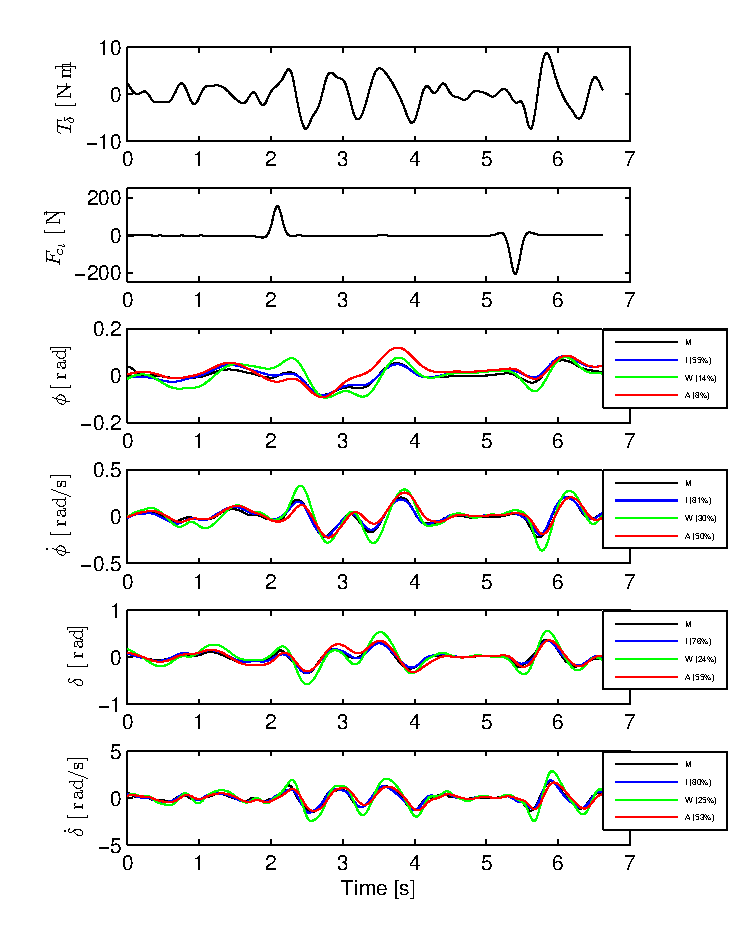
\includegraphics{figures/systemidentification/example-fit.*}

The identified models are almost always unstable due to the high weave critical
speed and, even though the measured inputs stabilize the true system, they will
not necessarily stabilize the models. This poses an issue when gauging the
model quality by the percent variance of the output data explained by the model
(VAF variance accounted for [by the model]). A model that blows up during the
simulation may not necessarily be a bad model, but it will return a very small
percent variance and lose its ability to be compared by that criterion.
\cite{Biral2003} and \cite{Teerhuis2010} both are able to run feed-forward
simulations of their motorcycle models with the measured steering torque. They
both are dealing with high speed motorcycles which typically only have a
slightly unstable capsize mode. \cite{Teerhuis2010} uses a controller to
compensate the torque for unbounded errors so that the simulation doesn't blow
up. The method I use here is to choose short duration portions of the runs for
simulation and search for the best set of initial conditions to keep the model
stable during the duration. This generally works but there are ultimately some
incomparable runs due to this issue.

We use this structured state space output error identification procedure
for a collection of experiments ($n=368$) over a range of speeds between
about 1 and 9 m/s. Figures 11.8\textless{}figACoefficients\textgreater{}
and 11.9\textless{}figBCoefficients\textgreater{} plot the identified
coefficients of the dynamical equations of motion (i.e. the bottom two
rows of the $\mathbf{F}$ and $\mathbf{G}$ matrices) as a function of
speed for all of the experiments using box plots. Both the Whipple
(green) and arm (red) model predictions are superimposed for comparison.

The first notable thing is that the coefficients seem to generally have
large variance, especially as the speed increases. Secondly, the roll
acceleration, $\ddot{\phi}$, equation seems to be better predicted by
the two models and the data has less spread at the lower speeds, barring
the $\dot{\phi}$ coefficient which has large spread and no apparent
relationship with speed for both equations. The roll equation also seems
to have less spread in the experimental data. For example, the
$a_{\ddot{\phi}\delta}$ coefficient appears to be very tight and the
first principles models predict it very well. The constant, linear, and
quadratic trends in the coefficients are somewhat visible in the data
but the variance in the coefficients clouds it. This variability in the
coefficient predictions depends on many things including data quality,
the ability to identify a process noise model, speed being constant
during the run, choice of unknown coefficients, and more. With all of
these improved, detailed regression models may be able to reveal the
true trends. Nonetheless, these
graphs reveal several important things:

\begin{itemize}
  \item
    The identified models predict the data well with most having mean
    predicted variance of the four outputs above 70\% (but this is tightly
    coupled to run duration, i.e. longer runs have more room for model
    error).
  \item
    Some of the coefficients are well predicted by the Whipple model and
    can be fixed from first principles calculations, notably:
    $a_{\ddot{\phi}\phi}$, $a_{\ddot{\phi}\delta}$ and
    $b_{\ddot{\delta}T_\delta}$ and maybe even $a_{\ddot{\delta}\delta}$.
  \item
    The roll rate coefficients are highly variable with poor prediction by
    the models. Deficiencies in the first principles models are likely.
  \item
    Either the higher speed runs are outliers, or the behavior of the
    system changes more rapidly with speeds above 5 m/s or so.
  \item
    Some coefficients spread around zero giving inconsistent signs and
    others give opposite signs from those the first principles models
    expect.
\end{itemize}

%\includegraphics{figures/systemidentification/a-matrix-box-plot.*}

%\includegraphics{figures/systemidentification/b-matrix-box-plot.*}

Figure 11.10\textless{}figStateSpaceBode\textgreater{} is a frequency 
response plot at the mean speed for a set of runs. The blue lines give the mean and one standard
deviation bounds of the magnitude and phase of the system transfer
function $\frac{\phi}{T_\delta}(s)$ for the set of runs. Even though the
spread in the identified parameters seems high in Figures
11.8\textless{}figACoefficients\textgreater{} and
11.9\textless{}figACoefficients\textgreater{}, the Bode plot shows that
the identified system frequency response is not as variable, especially
in magnitude. It is also apparent that the experimental magnitude mean
has a -5 to -10 dB offset across the frequency range shown with respect
to the Whipple model, although the Whipple model does fall within one
standard deviation of the mean. This correlates with the amplitude
differences in the trajectories shown in
Figure 11.7\textless{}figExampleFit\textgreater{}. Notice that the arm
model has little to no offset between 2 and 10 rad/s, thus the better
amplitude matching. The frequency response may give a better indication
of the overall identified model quality.

%\includegraphics{figures/systemidentification/state-space-bode.*}

\section{Canonical Identification}
\label{sec:canonical-identification}

% TODO : latex doesn't deal with unicode in karl's name

We obtained the system identification with respect to the second order form of the equations of
motion, an idea proposed to us by Karl Åström. This would allow one to use both
simple least squares for the solution and the ability to compute models from
large sets of runs. 

\subsection{Model structure}

Identification of bicycle linear dynamics can be formulated with
respect to the augmented benchmark canonical form realized in
\cite{Meijaard2007}, Equation \ref{eq:canonical}. If the time varying
quantities in the equations are all measured at each time step, the
coefficients of the linear equations can be estimated given enough time steps.

\begin{equation}
  \mathbf{M} \ddot{q} + v \mathbf{C}_1 \dot{q} + [g \mathbf{K}_0 + v^2
  \mathbf{K}_2] q = T + H F
  \label{eq:canonical}
\end{equation}

where the time-varying states roll and steer are collected in the vector $q =
[\phi \quad \delta]^T$, the time varying inputs roll torque and steer torque
are collected in the vector $T = [T_\phi \quad T_\delta]^T$, and $H = [H_{\phi
F} \quad H_{\delta F}]^T$ is a vector describing the linear contribution of the
lateral force, $F$, to the roll and steer torque equations. This equation
assumes that the speed, $v$, is constant with respect to time as the model was
linearized about a constant speed equilibrium, but we treat $v$ as a time
varying parameter because the measured longitudinal acceleration is negligible.
The augmented form extends the equations in \cite{Meijaar2007} to properly
account for the lateral perturbation force, $F$, which was the actual input we
delivered during the experiments. The force was applied just below the seat so
most of the contribution from $F$ is in the roll equations.

\subsection{Data Preprocessing}

The signals were measured and processed as described in Section \ref{sec:} with
the addition that the roll and steer accelerations were estimated by
numerically differentiating the roll and steer rate signals.

\subsection{Identification}

A simple analytic identification problem can be formulated from the canonical
form. If we have good measurements of $q$, their first and second derivatives,
forward speed $v$, and the inputs $T_\delta$ and $F$, the entries in
$\mathbf{M}$, $\mathbf{C}_1$, $\mathbf{K}_0$, $\mathbf{K}_2$, and $H$ can be
identified by forming two simple linear regressions (one for each equation
in the canonical form).

The roll and steer equations each can be put into a simple linear form:

\begin{equation}
  \mathbf{\Gamma} \Theta = Y
\end{equation}

where $\Theta$ is a vector of the unknown constant matrix entries and the
design matrix, $\mathbf{\Gamma}$, and the prediction vector, $Y$, are made up
of the inputs and outputs measured during a run. $\Theta$ can be all or a
subset of the entries in the canonical matrices. $\hat{\Theta}$ can be
estimated using the well known linear least squares solution.

\begin{equation}
  \hat{\Theta} = [\mathbf{\Gamma}^T \mathbf{\Gamma}]^{-1} \mathbf{\Gamma}^T Y
  \label{eq:theta-estimate}
\end{equation}

The error in the fit, i.e. residuals, is

\begin{equation}
  \epsilon = \hat{Y} - Y = \mathbf{\Gamma} \hat{\Theta} - Y
  \label{eq:fit-error}
\end{equation}

The covariance of the parameter estimations $\hat{\Theta}$ can be computed with
respect to the error.

\begin{equation}
  \sigma^2 = \frac{\epsilon^T\epsilon}{N - d} \\
  \label{eq:fit-variance}
\end{equation}

\begin{equation}
  \mathbf{U} = \sigma^2 (\mathbf{\Gamma}^T \mathbf{\Gamma})^{-1}
  \label{eq:theta-covariance}
\end{equation}

where $d$ is the degrees of freedom and $N$ is the number of something.

Equations \ref{eq:theta-estimate}, \dots \ref{eq:theta-covariance} can be
solved for each run individually, a portion of a run, or a set of runs.
Secondly, all of the parameters in the canonical matrices need not be
estimated. The analytical formulation of the Whipple model bicycle model
\cite{Meijaard2007} gives a good idea of which entries in the matrices we may
be more certain about from our physical parameters measurements. We fixed the
parameters if it is a function of trail, front assembly moments and products of
inertia, or equal to zero. Because the true trail is difficult to measure, the
inertia of the front frame play a large roll in the steer dynamics.

For the roll equation this leaves $M_{\phi\delta}$, $C_{1\phi\delta}$,
and $K_{0\phi\delta}$ as free parameters, and for the steer equation
this leaves $M_{\delta\phi}$, $M_{\delta\delta}$, $C_{1\delta\phi}$,
$C_{1\delta\delta}$, $K_{0\delta\phi}$, $K_{0\delta\delta}$,
$K_{2\delta\delta}$, and $H_{\delta F}$ as free parameters.

We start by identifying the three coefficients of the roll equation for
the given data using

\begin{align}
  &\begin{bmatrix}
     \ddot{\delta}(1) &
     v(1) \dot{\delta}(1) &
     g \delta(1) \\
     \vdots & \vdots & \vdots\\
     \ddot{\delta}(N) &
     v(N) \dot{\delta}(N) &
     g \delta(N) \\
  \end{bmatrix}
  \begin{bmatrix}
    M_{\phi\delta} \\
    C_{1\phi\delta} \\
    K_{0\phi\delta}
  \end{bmatrix}\\
  &=
  \begin{bmatrix}
    H_{\phi F} F(1)
    - M_{\phi\phi} \ddot{\phi}(1)
    - C_{1\phi\phi} v(1) \dot{\phi}(1)
    - K_{0\phi\phi} g \phi(1)
    - K_{2\phi\phi} v(1)^2 \phi(1)
    - K_{2\phi\delta} v(1)^2 \delta(1) \\
  \vdots\\
    H_{\phi F} F(N)
    - M_{\phi\phi} \ddot{\phi}(N)
    - C_{N\phi\phi} v(N) \dot{\phi}(N)
    - K_{0\phi\phi} g \phi(N)
    - K_{2\phi\phi} v(N)^2 \phi(N)
    - K_{2\phi\delta} v(N)^2 \delta(N) \\
  \end{bmatrix} \nonumber
\end{align}

We then enforce the assumptions that $M_{\phi\delta} = M_{\delta\phi}$ and
$K_{0\phi\delta} = K_{0\delta\phi}$ to fix these values in the steer equation
to the ones identified in the roll equation, leaving fewer free parameters in
the steer equation. Finally, I identify the remaining steer equation
coefficients with

\begin{align}
  \begin{bmatrix}
    \ddot{\delta}(1) &
    v(1) \dot{\phi}(1) &
    v(1) \dot{\delta}(1) &
    g \phi(1) &
    v(1)^2 \delta(1) &
    - F(1)\\
    \vdots & \vdots & \vdots & \vdots & \vdots & \vdots \\
    \ddot{\delta}(N) &
    v(N) \dot{\phi}(N) &
    v(N) \dot{\delta}(N) &
    g \phi(N) &
    v(N)^2 \delta(N) &
    - F(N)\\
  \end{bmatrix}
  \begin{bmatrix}
    M_{\delta\delta} \\
    C_{1\delta\phi} \\
    C_{1\delta\delta} \\
    K_{0\delta\phi} \\
    K_{2\delta\delta} \\
    H_{\delta F}
  \end{bmatrix} \nonumber \\
  =
  \begin{bmatrix}
    T_\delta(1)
    - M_{\delta\phi} \ddot{\phi}(1)
    - K_{0\delta\delta} g \delta(1)
    - K_{2\delta\phi} v(1)^2 \phi(1) \\
    \vdots\\
    T_\delta(N)
    - M_{\delta\phi} \ddot{\phi}(N)
    - K_{0\delta\delta} g \delta(N)
    - K_{2\delta\phi} v(N)^2 \phi(N) \\
  \end{bmatrix}
\end{align}

\subsection{Results}

I selected data for three riders on the same bicycle, performing two
maneuvers, in two different environments. I opted to compute the best fit model across series
of runs to benefit from the large dataset and to take into account variation across riders. 
This leaves these four scenarios with a total of 12 different models:

\begin{itemize}
  \item
    All riders in both environments, one data set
  \item
    All riders in each environment, two data sets
  \item
    Each rider in both environments, three data sets
  \item
    Each rider in each environment, six data sets
\end{itemize}


\subsubsection{All riders in both environments}

This section details the example results for one subset of data. Here I
make the assumption that the best fit model doesn't vary much across
riders or environments. This assumption can be justified by
recognizing the Whipple model predicts little difference in
dynamics with respect to the three bicycle/rider combinations. I
calculated the best fit over 374 runs giving about 142 minutes of data
sampled at 200 Hz, $N=1720647$.

The eigenvalues as a function of speed of the identified model can be
compared to those of the Whipple and arm models (see Section
secRiderArms in Chapter Extensions).
Figure 11.11\textless{}figAARloc\textgreater{} shows the root locus of
the three models. The oscillatory weave mode exists in all three models,
stable at all speeds in the arm model but unstable at lower
speeds in the other two models. The identified model's oscillatory weave
mode is unstable over most of the shown speed range. Above 3 m/s or so,
the Whipple model's oscillatory weave mode diverges from the identified
model to different asymptotes. The arm model weave mode diverges
somewhere in between. Note that the arm model has an unstable real mode
for all speeds. Figure
11.12\textless{}figAAEig\textgreater{} gives a different view of the
root locus allowing one to more easily compare the real parts of the
eigenvalues. The imaginary parts of the weave mode have similar
curvature with respect to speed for all the models, with the identified
model having about 1 rad/s larger frequency of oscillation for all
speeds. The identified model does have a stable speed range where the
Whipple model under predicts the weave critical speed by almost 2 m/s.
The identified caster mode is much faster than the one predicted by the
Whipple model which is somewhat counterintuitive because tire scrub
torques would probably tend to slow the caster mode. Although, the
pneumatic trail and the rider's arm inertia could play a larger role
that expected. Furthermore, the caster mode may not be well identified
because the experiments were not design to specifically excite it.

%\includegraphics{figures/systemidentification/A-A-rlocus.*}

%\includegraphics{figures/systemidentification/A-A-eig.*}

The identification process is based on identifying the input/output
relationships among measured variables. The frequency response provides
a view into these relationships. Figures
11.13\textless{}figAATphiPhi\textgreater{} to
11.16\textless{}figAATdelDel\textgreater{} give a picture of how the
first principles models compare to the identified model with respect to
frequency response from a roll torque input. The frequency band from 1
rad/s to 12 rad/s is of most concern as it bounds a reasonable range
that the human may be able to operate within.

The roll torque to roll angle response
Figure 11.13\textless{}figAATphiPhi\textgreater{} shows that at 2 m/s
(solid lines) the response of the Whipple model and the identified model
are practically identical across the frequency range shown. On the other
hand, the arm model predicts the high frequency (\textgreater{} 4 rad/s)
behavior really well, but the magnitude is as great as 50 dB larger and
the phase off by 180 degrees at lower frequencies. At 4 m/s the Whipple
model still predicts the phase well, but the magnitudes do not match
below 100 rad/s with 10 dB difference at lower frequencies. At this
speed the arm model matches the identified model as low as 3.5 rad/s but
the low frequency phase still being 180 degrees off. The magnitude of
the identified model stays quite constant among the 4, 6, and 9 m/s
models. As the speed increases the Whipple and arm models are less
predictive of the identified model at low frequencies, but tend to match
out past 4 rad/s or so.

%\includegraphics{figures/systemidentification/A-A-Tphi-Phi.*}

Figure 11.14\textless{}figAATphiDel\textgreater{} shows the steer angle
response with respect to the roll torque. Once again the Whipple model
is almost identical to the identified model at the lowest speed, 2 m/s.
The arm model has about a +5 dB offset at low frequencies and a -10 dB
offset at high frequencies with the models only being similar just
around 4 rad/s. At 9 m/s the Whipple model has similar magnitude and
phase above 7 rad/s whereas the low frequency shows that the Whipple
model has up to +30 dB magnitude difference with respect to the
identified model. The arm model behaves in much the same way at 9 m/s.

%\includegraphics{figures/systemidentification/A-A-Tphi-Del.*}

The steer torque to roll angle transfer function, Figure
11.15\textless{}figAATdelPhi\textgreater{} may be the most important to
model accurately as it is the primary method of controlling the
bicycle's direction, i.e. commanding roll allows one to command yaw. At
2 m/s the Whipple model magnitude matches at lower frequencies
(\textless{} 4 rad/s) better and the arm model better at higher
frequencies (\textgreater{} 4 rad/s). A 4 m/s and above the magnitude of
identified varies little with speed, which contrasts the stronger speed
dependence of the first principles models. The low frequency behavior of
the identified model is not well predicted by the Whipple and arm models
at the three highest speeds but about about 3 rad/s the arm model shows
better magnitude matches than the Whipple model.

%\includegraphics{figures/systemidentification/A-A-Tdel-Phi.*}

The steer torque to steer angle frequency response, Figure
11.16\textless{}figAATDelDel\textgreater{}, shows that at speeds above 2
m/s the first principle models do not predict the response well at low
frequencies. The response changes more drastically with respect to speed
for the first principles models than for the identified model.

%\includegraphics{figures/systemidentification/A-A-Tdel-Del.*}

\subsubsection{Comparison of identified models}

Tables 11.3\textless{}tabIdMCKOne\textgreater{},
11.4\textless{}tabIdMCKTwo\textgreater{}, and
11.5\textless{}tabIdMCKThree\textgreater{} present the identified
canonical coefficient values from all twelve of the chosen data subsets.
The variances of the coefficient estimates with respect to how well the
model fits the data in the steer equation are quite low except for the
$H_{\delta F}$ parameter. The low variance is partially due to the large
datasets but also due to the quality of the resulting fits. The
$H_{\delta F}$ is highly dependent on the trail which is expected to be
difficult to identify. The coefficient estimates are not all repeatable
among the data subsets. In particular $C_{1\delta\phi}$ and
$H_{\delta F}$ have the largest relative variance among the models
(\textgreater{} 62\%). $M_{\delta\delta}$, $C_{1\phi\delta}$,
$C_{1\delta\delta}$, and $K_{2\delta\delta}$ are the most consistent
among the models (\textless{} 18\%) with the remaining coefficients
falling somewhere in between. This is odd because these data sets are
not independent of one another; however, the identification procedure 
does not explicitly account for process noise. A sensitivity
study for each physical parameter coefficient could reveal which parameters
are less likely fit into the Whipple model.

It is interesting to note $C_{1 \delta \phi}$ deviates quite
significantly from the Whipple model prediction. This term depends on
the wheel radii, wheel rotational inertia, wheelbase, steer axis tilt,
and trail. 

\[c = -\frac{w(C_{1 \delta \phi} + S_F \operatorname{cos}\lambda)}{S_T
\operatorname{cos}\lambda}\]

The results for each data subset are given in Table
11.6\textless{}tabIdentifiedTrail\textgreater{}. On average, the values
are unrealistic compared to the measured geometric trail
of $c=0.0599$ meters. This may imply that including the effects of
pneumatic trail does not sufficiently improve the predictive
capabilities of the Whipple model. The data also point to the potentially
erroneous assumptions made in this identification effort such as the
order of the system and which parameters are fixed. Although the
model adequately describes the measured motion, it lacks the
complexness to identify the precise deficients in the first principles
assumptions.

The measurement errors, model structure and order dictate how well the
models can predict the input-output behavior of each run or even each
perturbation. The previous section's state space methods have already 
shown that the Whipple and arm models may not provide adequate predictions.

Figures 11.17\textless{}figCompBode2p0\textgreater{},
11.18\textless{}figCompBode5p5\textgreater{}, and
11.19\textless{}figCompBode9p0\textgreater{} plot the steer torque to
roll angle frequency response for three speeds: 2 m/s, 5.5 m/s and 9.0
m/s for each of the models in Tables
11.3\textless{}tabIdMCKOne\textgreater{},
11.4\textless{}tabIdMCKTwo\textgreater{}, and
11.5\textless{}tabIdMCKThree\textgreater{}. At the lowest speed, all models 
have a similar frequency response particularly in the
frequency band between 1 and 20 rad/s. At 5.5 m/s the models are
similar at a higher bandwidth (4 to 30 rad/s), and at 9.0 m/s even
higher (10 to 50 rad/s). The model derived from all of the data (all rider and all runs), gives an
average model. If this model is significantly better at predicting
the measured behavior of the Whipple and arm models, it may be a good
general candidate model for this bicycle.

%\includegraphics{figures/systemidentification/compare-id-bode-2p0.*}

%\includegraphics{figures/systemidentification/compare-id-bode-5p5.*}

%\includegraphics{figures/systemidentification/compare-id-bode-9p0.*}

The predictive capability and quality of a given model can be quantified
by an assortment of criteria and methods. Two criteria used to judge 
the quality of these models with respect to given data are (1) simulate 
the system given the measured inputs. This method works well when the open loop system is stable, but if it is
unstable as so in the case of this bicycle, it may be difficult to
simulate. Searching for initial conditions that give rise to a stable
model for the duration of the run or simulating by weighting the future
error less may relieve the instability issues. (2) See
how well the inputs are predicted given the measured outputs. The
canonical form of the equations lend themselves to this and only two
inputs per run need be checked.

The predicted torques on the system are

\[y_p = \mathbf{M} \ddot{q} + v \mathbf{C}_1 \dot{q} + [g \mathbf{K}_0 + v^2
\mathbf{K}_2] q\]

and the measured torques as

\[y_m = T + H F\]

$y_p$ and $y_m$ can be computed for each run along with the
\emph{variance accounted for} (VAF), by the model for both the total
roll torque and the steer torque

\[\textrm{VAF} = 1 - \frac{\vert \vert y_p - y_m\vert \vert }{\vert \vert y_m - \bar{y}_m\vert \vert }\]

I compute the VAF for each of the 374 runs used in the canonical
identification outlined in Equation eqVAF using each of the 12
identified models and both the Whipple and Arm models. This percentage
can be used as a criterion to judge the ability of one model
versus another to predict the measurement. I then take the median of the
VAF over each of the 12 sets of runs, Tables
11.7\textless{}tabMeanVAFRoll\textgreater{} and
11.8\textless{}tabMeanVAFSteer\textgreater{}. The results give an idea
of how well the various models are able to predict the data for all of
the runs in a given set.

Tables 11.7\textless{}tabMeanVAFRoll\textgreater{} and
11.8\textless{}tabMeanVAFSteer\textgreater{} give the median for each
set of runs in each column for each model given in the row for roll and
steer respectively. The maximum VAF in the column gives a measure of the
best model for predicting each individual run in that set of runs.
Intuitively, I would expect that the diagonal of the upper 12 rows would
be the maximum in each column due to the fact that that model was
derived from that set of runs, but that is not always the case. I
believe that this can be explained by the fact that there are more
outlier runs in some sets. These outliers have enough effect in the
resulting regressions, that the models generated from sets of runs with
fewer outliers are able to predict the data better.

The models are able to predict the steer torque much better than the
roll torque. The roll torque should be zero in all of the runs without
disturbances but the roll equations do not predict a zero value. This is
also reflected in the negative median values of all the runs with
disturbances in much of
Table 11.7\textless{}tabMeanVAFRoll\textgreater{}. We fixed six of the
nine parameters in the roll equation to those of the Whipple model and
fixed three of the nine parameters in the steer equation. These extra
degrees of freedom explain why the steer predictions are
better than the roll predictions. The model for the roll torque is more
susceptible to noise in rate and angle measurements with variation of
+/- 50 Nm in the predicted roll torques. These
are unfortunately comparable in magnitude to the measured roll torques
due to lateral perturbations. But Table
11.7\textless{}tabMeanVAFRoll\textgreater{} can still be used to gauge
which models are better with reference to each other. Values in
Table 11.7\textless{}tabMeanVAFRoll\textgreater{} are only generated
from runs with disturbances, as a relative measure of quality to
zero is difficult to make.

Tables 11.7\textless{}tabMeanVAFRoll\textgreater{} and
11.8\textless{}tabMeanVAFSteer\textgreater{} reveal:

\begin{itemize}
  \item
    The arm model is poor at predicting the steer torque.
  \item
    The models derived from Charlie's runs are poorer at predicting the
    inputs.
  \item
    The Whipple model is not too bad at predicting steer torque, but on
    average about 10\% worse than the best models.
  \item
    The models identified from the pavilion runs are generally the best
    (with exception of Charlie's). The ones generated from Luke and
    Jason's runs are typically the best at predicting both steer torque
    and roll torque, with Luke's giving better roll torque predictions.
  \item
    The roll torque is poorly predicted by all models when it is supposed
    to be zero. This raises implications in the validity of the roll
    equation and the potential need for tire slip models.
\end{itemize}

It may seem odd that a model identified from the subset of runs of one
rider in one environment is the best at predicting the runs on a
individual basis, but the uncertainty and error in both the data and the
model structures don't dictate that this can't be. %holy crap long ass sentence
keep in mind that the frequency responses of all 12 models shown in Figures
11.17\textless{}figCompBode2p0\textgreater{},
11.18\textless{}figCompBode5p5\textgreater{}, and
11.19\textless{}figCompBode9p0\textgreater{} are probably bounded in the
uncertainty of the predicted responses and each can be considered a
``good'' model, even including the Whipple model.

The second method of evaluating the quality of the identified models is
to simulate the model with the measured inputs and compare the predicted
outputs with the measured outputs with a similar VAF criterion. I
simulated all 14 models with the inputs from the 374 runs and computed
the VAF explained by the model for each output. Since the models are
typically unstable at all of the speeds we tested, I searched for the
set of initial conditions which minimizes the VAF for all outputs. For
the majority of runs and models, this is sufficient to find a stable
simulation for the duration of the run. However, this is not always the
case. For long duration runs I select a random 20 second section of the
data to simulate, reducing the likelihood that the simulation blows up
due to the model's instability. Finally, I ignore any outputs VAFs that
are less than -100 percent as they are most likely due to unstable
simulations. Table 11.9\textless{}tabMedianVAFOutputs\textgreater{}
presents the median percent variance accounted for across all runs for
each model and each output. The best model seems to be the one generated
from the data with Luke on the Pavilion Floor once again, but these
results differ from the previous otherwise. %can you make this paragraph more consice?

\begin{itemize}
  \item
    For all outputs other than roll angle, the arm model is better than
    the Whipple model.
  \item
    The models from Charlie's data fare much better than the input
    comparisons and are better than some of Jason's.
  \item
    The model identified from the data with Jason on the Pavilion floor is
    very poor in roll angle prediction as opposed to being a good choice
    from the input comparison results.
  \item
    All of the identified models are better predictors than the first
    principles models.
\end{itemize}

The mean percent variance across the outputs can be computed and the
models ranked by the mean,
Table 11.10\textless{}tabMeanVAFOutputs\textgreater{}. The best model
seems to be LP and the AA is also a pretty good predictor. Notice that
the Whipple model is poorer than the arm model.

The orange lines in Figures
11.8\textless{}figACoefficients\textgreater{} and
11.9\textless{}figBCoefficients\textgreater{} correspond to the L-P
model which allows comparison of the results of the canonical
identification process with those of the state space identified models.
The L-P model seems be better at fitting the data, especially in the
steer acceleration equation, but the large variance in the state space
coefficients is still a problem. This lends more confidence that that
the L-P model is a better model choice than the Whipple or the arm
model.

\section{Discussion}

We have shown that a fourth order linear model is adequate for describing the
motion of the bicycle under manual control in a speed range from approximately
1.5 m/s to 9 m/s. Results from this study show that a higher order models may not be necessary for
predicting the bicycle-rider dynamics. This is an important finding, as many
researchers develop models using first principles which have orders much greater
than 4, with degrees of freedom associated with tire slip, frame flexibilities,
and rider biomechanics, which may be overkill for many prediction purposes. But, results 
also reveal that fourth order archetypal first principles models are not
predictive enough to fully describe the dynamics. These deficiencies are most 
likely due to un-modeled effects, with knife-edge, no side-slip wheel contact 
assumptions being the most probable candidate. Un-modeled rider biomechanics such as passive arm stiffness and
damping and head motion may play a role too. It is likely that something as
simple as a ``static'' tire scrub torque is needed to improve the fidelity of
the Whipple first principles derivations, but that doesn't preclude that the
addition of a tire slip model, adding more degrees of freedom, might also
improve the predictive ability.

\subsection{Canonical identification}

The canonical realization Section secCanonicalId, % is this a code?
is a good method for identifying a model using data from multiple runs, as it relies 
on quality measurements of the coordinates, rates, and accelerations. Rather than 
direct measurements, we relied on numerical differentiation of the rates to get the accelerations. 
Furthermore, differentiation of the measured angles do not exactly reproduce the 
measured rates because they were measured from different
sensors. Using a sensor fusion algortm could The noise in the measurements and
whether the measurements are accurately the derivatives of one another have
bearing on the results.%sentense does not make sense. 

It is possible to identify all of the entries in the canonical matrices, but it
is likely some of those are easily predicted from first principles so we fixed
them to the Whipple model predictions if that is the case. %whoa what? fix
This leaves the roll equation mostly known and the steer equation mostly unknown and the results
reflect better fits with respect to steer than roll as a result. %fix

This formulation does not explicitly account for process noise, so it may be be
susceptible to similar accuracy errors as the state space formulation is. %fix or delete
The advantage in this method is the ability to use large sets of data for the
calculations. It is extremely surprising that a model from a small subset of
the data is better at predicting all of the runs on an individual basis.

\subsection{Input comparison}

The input prediction comparisons do not predict the roll torque well. The roll torque equation magnifies the noise in the coordinate,
rate and acceleration measurements such that the resulting noise in the roll
torque is equivalent in magnitude to the roll perturbations. But the roll
perturbations do seem to clearly be present in the predictions. This results in
difficultly comparing the quality of the resulting models with respect to the
roll equation. This also points to the potential deficiencies in the Whipple
roll torque equation and these large magnitude roll torques may also be due to
inaccurate modeling of the tire dynamics. %this may be written better...

\subsection{Output comparison}

The output comparisons (simulations) give more reasonable results because
all four outputs generally fit well across runs. It is surprising that the ranking of model prediction ability is
different for the input comparisons than the output comparisons, but the
fact that the model identified from Luke's pavilion runs is the best
from both comparisons, at least gives credence to its further adoption. %err....fix? OR can this whole section go?
The first principles models are dead last in the ranking and the model
identified from Jason's pavilion runs is surprisingly poor due to poor
roll angle prediction.

\subsection{Whipple model}

The input comparisons show that the Whipple model is relatively
reasonable at predicting the data but the output comparisons make it out
to be much poorer. The Whipple model is clearly the worst at explaining
variance in the steer angle, roll rate, and steer rate outputs and
is second to worst in roll angle. Also, contrary to the Whipple model
predictions, the weave mode of all identified models is unstable until
at least 8-9 m/s. The caster mode is also typically much faster in
the identified models, implying the real system does not
benefit from open loop stability during most normal speed
bicycling and that the rider is always responsible for stabilizing the
vehicle. 

\subsection{Arm model}

We had hypothesized that the arm model would better predict the measured
motion because it more accurately modeled the fact that we allowed the
rider full use of his arms to control the steering and that the arms
effectively added to the front frame inertia. The output simulation 
comparisons validated this hypothesis as they predict the arm
model is much better than the Whipple model for most output
variables. This is in contrast to the input comparison predictions, which states the Whipple
to be much better than the arm model. More work is needed to verify which model is better and why the
results differ at all.

\subsection{Rider biomechanics may mot be modeled}

The models identified from Charlie's runs differ to those of Jason and
Luke and do not predict the runs very well, even when including the subset 
of Charlie's data. I'm not sure whether the rider's arm
stiffness or difference in riders could have effected
this if we are only searching for the passive bicycle-rider model. There also 
could have been too many outliers in Charlie's runs, related to those that had time synchronization
issues.

\subsection{Predicting derivatives}

The steer angle and steer rate are better predicted than the roll angle and
roll rate.  The poorer
prediction of roll angle is probably due to noise and error in the
independent measurements of these variables. I toyed with complementary
filters to try to combine the angle and rate measurements in a way that
filtered and enforced the derivative relationship between the measured
variables, but did not have much luck improving the results. It may be
better to focus on one each of the roll and steer variables for
minimization purposes. It is well known that fitting models with many
fewer inputs to outputs is difficult and the fewer outputs reduces the
number of noise terms to estimate.

The best candidate model for the measured system is the model identified
from the data subset with rider Luke and the pavilion floor. I find no
reason to use different models for each rider or environment as this
model does a better job at predicting than the other models derived from
matching subsets. I will use the model identified from the set of runs
with Luke on the pavilion floor as the base bicycle model for
identifying the controller for all the runs in the following section of
this Chapter. I could use the individual bicycle identifications for
each run, but using a model derived from a set of runs has the advantage
that it will be less affected by the lack of identifying the process
noise explicitly. %there is some repetitiaon in this paragraph, try and fix

Suggestions for improving the results.

\begin{itemize}
  \item
    Fit to MISO models instead of MIMO for simplification.
  \item
    Fix at least the $a_{\phi\delta}$ coefficient and make the noise with
    respect to the kinematical equations equal to zero giving 11-13 total
    parameters to fit.
  \item
    Use model reduction techniques to combine many MISO and SISO models
    for a given run.
  \item
    Use better initial guess techniques and try global optimizers to get
    to the best solution.
\end{itemize}

\section*{Acknowledgements}

This paper is based on work supported by the National Science Foundation under
Grant No 0928339. Karl Astrom gave me the ideas for the canonical form.

%\printbibliography

\bibliographystyle{plain}
\bibliography{references}

\end{document}
